\documentclass[11pt]{article}
\usepackage{amsmath,amssymb}
\usepackage{graphicx}

\begin{document}

\section{Gluing the temporal axis of a layer}

\subsection{Definitions}

\textbf{Definition 1 (category).} A category $\mathcal{C}$ consists of a class of objects; for every two objects $A,B$ a set $\mathcal{C}(A,B)$ of morphisms $f:A\to B$; for every object an identity morphism $\mathrm{id}_A$; and a composition $g\circ f:A\to C$ of $f:A\to B$ and $g:B\to C$, which is associative and has the identities as units (Mac Lane, \emph{Categories for the Working Mathematician}, Ch.~I). The category $\mathbf{Set}$ has sets as objects and functions as morphisms.

\textbf{Definition 2 (functor).} A functor $F:\mathcal{C}\to\mathcal{D}$ assigns to each object $A$ of $\mathcal{C}$ an object $F(A)$ of $\mathcal{D}$ and to each morphism $f:A\to B$ a morphism $F(f):F(A)\to F(B)$, so that $F(\mathrm{id}_A)=\mathrm{id}_{F(A)}$ and $F(g\circ f)=F(g)\circ F(f)$.

\textbf{Definition 3 (natural transformation).} Given functors $F,G:\mathcal{C}\to\mathcal{D}$, a natural transformation $\alpha:F\Rightarrow G$ is a family of morphisms $\alpha_A:F(A)\to G(A)$, one for each object $A$, such that $G(f)\circ\alpha_A=\alpha_B\circ F(f)$ for every $f:A\to B$.

\textbf{Definition 4 (diagram).} A diagram of shape $\mathcal{J}$ in $\mathcal{C}$ is a functor $D:\mathcal{J}\to\mathcal{C}$, where $\mathcal{J}$ is a small category. It is a family of objects $D(j)$ of $\mathcal{C}$ connected by the morphisms $D(u)$.

\textbf{Definition 5 (cocone and colimit).} A cocone under $D$ is an object $K$ with morphisms $\kappa_j:D(j)\to K$ such that $\kappa_{j'}\circ D(u)=\kappa_j$ for every $u:j\to j'$ in $\mathcal{J}$. A colimit of $D$ is a cocone $(K,\kappa)$ such that for every cocone $(N,\nu)$ there is exactly one morphism $h:K\to N$ with $h\circ\kappa_j=\nu_j$ for all $j$. It is written $\mathrm{colim}\,D$ and is unique up to a unique isomorphism (Mac Lane, Ch.~III).

A colimit is the most economical object into which every piece of the diagram maps compatibly: it glues the pieces together along what the diagram says they share, and adds nothing else.

\textbf{Definition 6 (pushout).} A pushout is a colimit of a diagram of shape $A\xleftarrow{f}C\xrightarrow{g}B$. In $\mathbf{Set}$ it is the disjoint union $A\sqcup B$ in which $f(c)$ and $g(c)$ are identified for every $c\in C$, and it is written $A\sqcup_C B$.

\textbf{Example.} Let $A=\{1,2\}$, $B=\{2,3\}$ and $C=\{2\}$, with $f$ and $g$ the inclusions. Then $A\sqcup_C B=\{1,2,3\}$: the two copies of $2$ are glued. If instead $C=\varnothing$, the pushout is the disjoint union $A\sqcup B$, which has four elements, since nothing is glued.

\textbf{Definition 7 (equivalence relation and quotient).} An equivalence relation $\sim$ on a set $X$ is a reflexive, symmetric and transitive relation. Its classes partition $X$; the quotient $X/{\sim}$ is the set of classes, and $\pi:X\to X/{\sim}$ sends each element to its class.

\textbf{Definition 8 (coequalizer).} A coequalizer is a colimit of a diagram of shape $A\rightrightarrows B$ with two morphisms $f,g$. In $\mathbf{Set}$ it is the quotient $B/{\approx}$ by the smallest equivalence relation with $f(a)\approx g(a)$ for all $a\in A$, together with the quotient map $B\to B/{\approx}$.

\textbf{Example.} Let $B=\{o_1,o_2,o_3\}$, $A=\{\ast\}$, $f(\ast)=o_1$ and $g(\ast)=o_2$. The coequalizer is $\{\{o_1,o_2\},\{o_3\}\}$: the map $f,g$ says that $o_1$ and $o_2$ are to be the same, and the coequalizer makes them so. Any equivalence relation $\sim$ on $B$ arises this way, by taking $A$ to be the set of pairs $(b,b')$ with $b\sim b'$ and $f,g$ the two projections.

\begin{center}
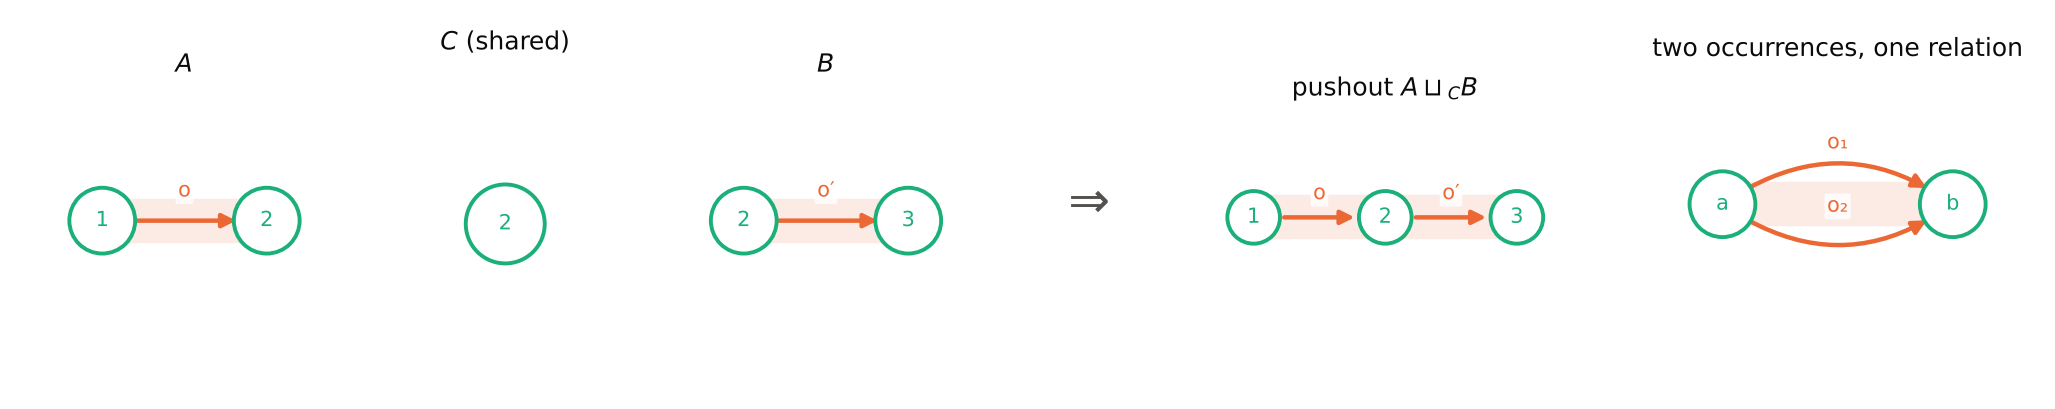
\includegraphics[width=\textwidth]{figs_gluing/g1_examples.png}

\textit{Figure 1. Left: the pushout of two hypergraphs sharing the vertex $2$ glues them into one. Right: two occurrences $o_1,o_2$ of an operation on the same variables; a coequalizer identifying them yields a single relation whose fibre is $\{o_1,o_2\}$.}
\end{center}

\subsection{The category of directed labelled hypergraphs}

\textbf{Definition 9 (schema).} Let $\Sigma$ be the category with four objects $V,E,I_s,I_t$ and, besides identities, four morphisms $\mathrm{se}:I_s\to E$, $\mathrm{sv}:I_s\to V$, $\mathrm{te}:I_t\to E$, $\mathrm{tv}:I_t\to V$.

\textbf{Definition 10 (directed hypergraph as a C-set).} A directed hypergraph is a functor $H:\Sigma\to\mathbf{Set}$ with finite values. $H(V)$ is the set of vertices, $H(E)$ the set of hyperedges; an element $i\in H(I_s)$ records that the vertex $H(\mathrm{sv})(i)$ is a source of the hyperedge $H(\mathrm{se})(i)$, and an element of $H(I_t)$ records a target in the same way. For a hyperedge $e$, its source set is $S(e)=H(\mathrm{sv})\big(H(\mathrm{se})^{-1}(e)\big)$, its target set is $T(e)=H(\mathrm{tv})\big(H(\mathrm{te})^{-1}(e)\big)$, and its vertex set is $V(e)=S(e)\cup T(e)$. A hyperedge of layer $1$ has exactly one target. This way of encoding combinatorial structures as functors on a schema is that of C-sets (Patterson, Lynch, Fairbanks 2022), and it is the one used by Bumpus et al.\ for temporal graphs.

Because hyperedges are elements of $H(E)$ and not subsets of $H(V)$, two different hyperedges may have the same sources and the same target. Two occurrences of an operation on the same variables are therefore two hyperedges.

\textbf{Definition 11 (morphism).} A morphism of directed hypergraphs $\alpha:H\to H'$ is a natural transformation: four functions $\alpha_V,\alpha_E,\alpha_{I_s},\alpha_{I_t}$ commuting with the four structure maps. It sends vertices to vertices and hyperedges to hyperedges, sources to sources and targets to targets, so it preserves direction.

\textbf{Definition 12 (labels).} A labelled directed hypergraph is a directed hypergraph together with a function $\tau:H(E)\to\mathcal{T}$ into a set $\mathcal{T}$ of terms; morphisms are required to satisfy $\tau'\circ\alpha_E=\tau$. The resulting category is written $\mathbf{DHyp}$.

\textbf{Proposition 1.} The category of functors $\Sigma\to\mathbf{Set}$ has all small colimits, computed objectwise: the colimit of a diagram of C-sets has as vertex set the colimit of the vertex sets, as edge set the colimit of the edge sets, and similarly for $I_s,I_t$, with the induced structure maps (Mac Lane--Moerdijk, \emph{Sheaves in Geometry and Logic}, Ch.~I). In the two colimits used below, hyperedges that are identified always carry the same label, so the labels pass to the colimit.

\textbf{Example.} The hyperedge $\{a,b\}\to c$ is the C-set with $H(V)=\{a,b,c\}$, $H(E)=\{o\}$, $H(I_s)=\{i_1,i_2\}$ with $\mathrm{sv}(i_1)=a$, $\mathrm{sv}(i_2)=b$, $\mathrm{se}(i_1)=\mathrm{se}(i_2)=o$, and $H(I_t)=\{j\}$ with $\mathrm{tv}(j)=c$, $\mathrm{te}(j)=o$.

\subsection{Gluing time: the occurrence hypergraph}

\textbf{Definition 13 (snapshot).} For a run of $A$ on $x$ with steps $t=1,\dots,T$, the snapshot $H_1^t$ is the labelled directed hypergraph with vertex set $V_t$ (the variables existing at step $t$), one hyperedge for each operation $o\in Op_t$, sources $S_o$, target $i_o$, and label $\tau_o$.

\textbf{Definition 14 (shared part).} For $1\le t<T$, the shared part $S^{t,t+1}$ is the hypergraph with vertex set $V_t\cap V_{t+1}$ and no hyperedges, together with its two inclusions $H_1^t\leftarrow S^{t,t+1}\rightarrow H_1^{t+1}$.

\textbf{Definition 15 (temporal diagram).} The temporal diagram of layer $1$ is the diagram
\[ H_1^1\leftarrow S^{1,2}\rightarrow H_1^2\leftarrow S^{2,3}\rightarrow\cdots\leftarrow S^{T-1,T}\rightarrow H_1^T \]
in $\mathbf{DHyp}$, whose shape is the zigzag with $T$ peaks and $T-1$ valleys.

\textbf{Definition 16 (occurrence hypergraph).} The occurrence hypergraph of layer $1$ is the colimit $O=\mathrm{colim}$ of the temporal diagram.

\textbf{Proposition 2 (explicit form).} Suppose that every variable exists on an interval of consecutive steps, as it does when it exists from the step that creates it to the end of the run. Then $O$ has vertex set $\bigcup_t V_t$, each variable once; hyperedge set $\bigsqcup_t Op_t$, each occurrence of an operation separately; and the sources, targets and labels of the snapshots.

\emph{Proof} (written for this section). By Proposition 1 the colimit is computed set by set. On vertices it is an iterated pushout of the $V_t$ along their consecutive intersections; a variable alive on the steps $a,\dots,b$ appears in each $V_t$ with $a\le t\le b$, and the copies are glued along each consecutive pair, so they become one element. On hyperedges and incidences the shared parts are empty, so each pushout is a disjoint union. $\square$

If a variable existed on two separate stretches of time, the colimit would keep two copies of it; the assumption excludes this.

$O$ is the value on the whole run $[1,T]$ of the cumulative narrative determined by the snapshots and their shared parts, in the sense of Bumpus et al., \emph{Towards a Unified Theory of Time-Varying Data} (Prop.~2.7 and 2.9). The step at which each occurrence happened is not kept in $O$; what is kept is that each occurrence is a distinct hyperedge.

\begin{center}
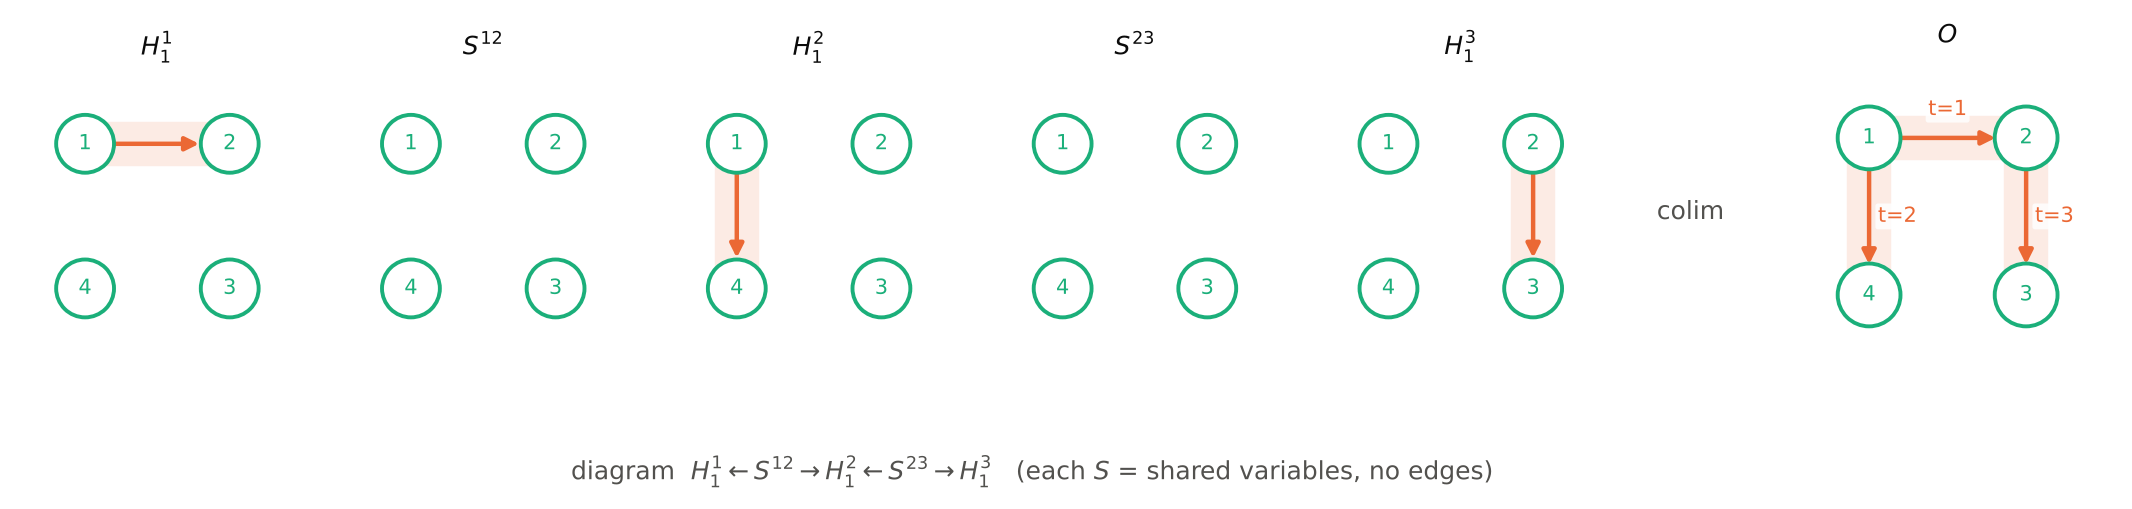
\includegraphics[width=\textwidth]{figs_gluing/g2_bfs_diagram.png}

\textit{Figure 2. BFS on $C_4$. The temporal diagram (five panels: three snapshots and the two shared parts, which contain all four variables and no hyperedge) and its colimit $O$, in which each of the three operation occurrences is a separate hyperedge.}
\end{center}

\subsection{Relations across the run: the relation hypergraph}

\textbf{Definition 17 (congruence).} A congruence on a C-set $H$ is a family of equivalence relations, one on each of $H(V),H(E),H(I_s),H(I_t)$, such that each structure map sends equivalent elements to equivalent elements.

\textbf{Proposition 3.} If $\equiv$ is a congruence on $H$, the objectwise quotient $H/{\equiv}$ is a C-set, and the quotient map $H\to H/{\equiv}$ is the coequalizer of the two projections from the C-set of equivalent pairs to $H$ (Proposition 1 applied to Definition 8).

\textbf{Definition 18 (occurrence rule).} An occurrence rule is an equivalence relation $\sim$ on the hyperedges of $O$ saying which occurrences count as the same relation. Three candidate rules are considered.
The \emph{directed rule}: $o\sim_{\mathrm{dir}}o'$ if and only if $S(o)=S(o')$ and $T(o)=T(o')$. It extends to a congruence on $O$ that fixes every vertex and identifies the source incidences of $o$ and $o'$ at the same vertex, and likewise for the targets.
The \emph{term rule}: $o\sim_{\mathrm{term}}o'$ if and only if $o\sim_{\mathrm{dir}}o'$ and $\tau(o)=\tau(o')$.
The \emph{vertex-set rule}: $o\sim_{\mathrm{vs}}o'$ if and only if $V(o)=V(o')$.

\textbf{Observation} (written for this section). The vertex-set rule does not in general extend to a congruence on $O$ that fixes the vertices. Identifying an occurrence $\{q\}\to e$ with an occurrence $\{e\}\to q$ would identify a source incidence at $q$ with a source incidence at $e$, and the structure map $\mathrm{sv}$ would then force $q$ and $e$ to be identified. The vertex-set rule is therefore applied to the undirected hypergraph $U(O)$ obtained by forgetting the distinction between sources and targets, which is a C-set on the schema with one incidence object.

\textbf{Definition 19 (relation hypergraph).} For an occurrence rule $\sim$ that extends to a congruence, the relation hypergraph is the quotient $R=O/{\sim}$ (or $U(O)/{\sim}$ for the vertex-set rule), with quotient map $\pi:O\to R$. For a relation $r$ of $R$, its fibre $\pi^{-1}(r)$ is the set of its occurrences and its multiplicity is $m(r)=|\pi^{-1}(r)|$.

Which rule defines ``the same relation'' is left open here; the construction is run below for all three.

\subsection{Extracting information: the algebra of $O$ and $R$}

\textbf{Definition 20 (toric ideal of a hypergraph with repeated hyperedges).} Let $H$ have vertices $v_1,\dots,v_n$ and hyperedges $e_1,\dots,e_r$, repeated vertex sets allowed. Let $\mathbb{Q}[x_1,\dots,x_n]$ have one variable per vertex, and $S_H=\mathbb{Q}[t_{e_1},\dots,t_{e_r}]$ one variable per hyperedge, graded by $\deg t_e=|V(e)|$. The toric ideal $I_H$ is the kernel of $\varphi_H:S_H\to\mathbb{Q}[x_1,\dots,x_n]$, $t_e\mapsto\prod_{v\in V(e)}x_v$ (Sturmfels, \emph{Gröbner Bases and Convex Polytopes}, Ch.~4; Petrović--Stasi). Its minimal generators are the relations among the interactions; the minimal graded free resolution of $S_H/I_H$, with its graded Betti numbers $\beta_{i,j}$, records the relations among those relations (Eisenbud; Peeva).

\textbf{Proposition 4} (written for this section). Let $\pi:O\to R$ be a quotient by an occurrence rule that preserves vertex sets, which is the case for all three rules. Let $\psi:S_O\to S_R$ be the ring map $t_o\mapsto t_{\pi(o)}$. Then $I_O=\psi^{-1}(I_R)$, and the kernel of $\psi$ is generated by the linear binomials $t_o-t_{o'}$ with $\pi(o)=\pi(o')$. In particular $I_R=\psi(I_O)$.

\emph{Proof.} Since $V(o)=V(\pi(o))$, we have $\varphi_O=\varphi_R\circ\psi$, hence $\ker\varphi_O=\psi^{-1}(\ker\varphi_R)$. The map $\psi$ is surjective and identifies variables, so its kernel is the ideal generated by the differences of the identified variables. $\square$

So the identifications made by an occurrence rule appear in the algebra of $O$ as linear binomials, and passing to $R$ removes them. The ordinary toric ideal sees only vertex sets: it cannot distinguish an occurrence from one with the same vertices and the opposite direction. For graphs, an oriented version exists: each oriented edge from $x_i$ to $x_j$ is given the column with $-1$ in position $i$ and $+1$ in position $j$ (Gitler, Reyes, Villarreal, \emph{Ring graphs and complete intersection toric ideals}). Its extension to hyperedges, and to operations that read and write the same variable, is not defined, and it is not used below.

\subsection{Running the construction on the three examples}

\paragraph{BFS.} The temporal diagram of $C_4$ is shown in Figure 2. $O$ has the four vertices and the three occurrences $\{1\}\to2$, $\{1\}\to4$, $\{2\}\to3$; on the domino it has the six vertices and five occurrences (Figure 3). No two occurrences have the same vertex set, so the three rules give $R=O$. The toric ideal is $I_O=0$ in both cases: the only nonzero Betti number is $\beta_{0,0}=1$. For comparison, layer $0$ of the same runs, the input graphs, has the toric ideal $(t_{12}t_{34}-t_{23}t_{14})$ for $C_4$ and an ideal with two generators and one syzygy for the domino.

\begin{center}
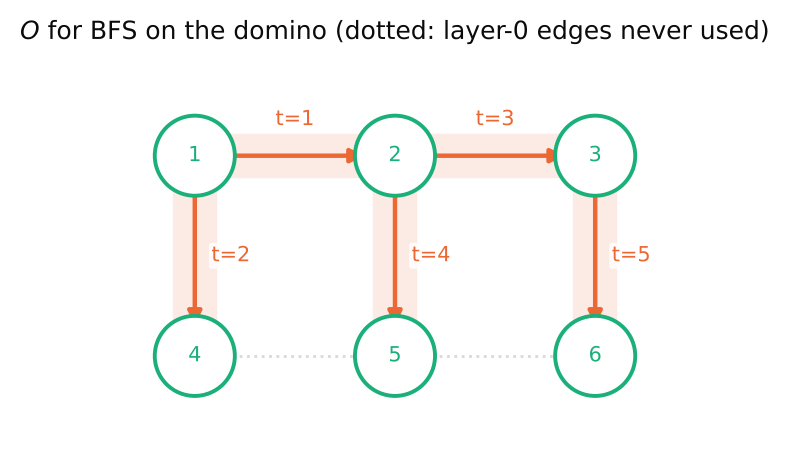
\includegraphics[width=0.6\textwidth]{figs_gluing/g3_bfs_domino_O.png}

\textit{Figure 3. The occurrence hypergraph of BFS on the domino. The dotted edges are edges of the input graph (layer $0$) that no operation uses.}
\end{center}

\paragraph{Teleportation.} $O$ has the seven variables $q_0,q_1,q_2,m_1,m_2,m_1',m_2'$ and the eight occurrences of the six steps (Figure 4, left). Their vertex sets are pairwise different, so the three rules give $R=O$. The toric ideal is principal:
\[ I_O=\big(\,t_{q_0}^2\,t_{q_1m_2}\,t_{m_1m_1'}\,t_{m_2'q_2}\;-\;t_{q_0q_1}\,t_{q_0m_1}\,t_{m_2m_2'}\,t_{m_1'q_2}\,\big), \]
homogeneous of degree $8$, with Betti numbers $\beta_{0,0}=1$ and $\beta_{1,8}=1$. Here $t_{q_0}$ is the Hadamard occurrence, $t_{q_0q_1}$ the CNOT, $t_{q_0m_1}$ and $t_{q_1m_2}$ the two measurements, $t_{m_1m_1'}$ and $t_{m_2m_2'}$ the two sendings, and $t_{m_2'q_2}$, $t_{m_1'q_2}$ the two corrections. Both sides of the binomial meet $q_0$ twice and every other variable once (Figure 4, centre and right): the Hadamard taken twice, one measurement, one sending and one correction balance the CNOT, the other measurement, the other sending and the other correction.

\begin{center}
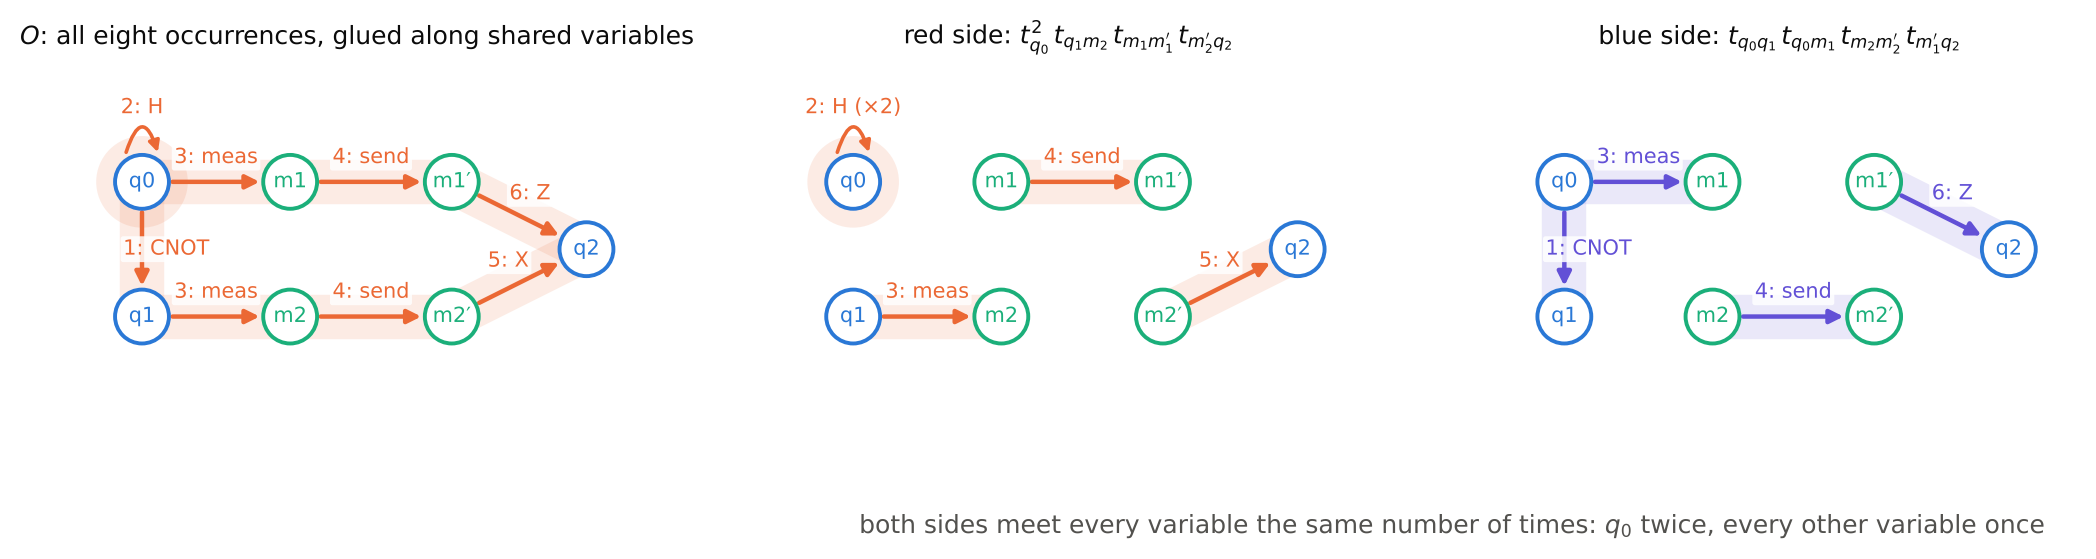
\includegraphics[width=\textwidth]{figs_gluing/g4_tele_O.png}

\textit{Figure 4. Teleportation. Left: the occurrence hypergraph $O$ (labels: step and operation). Centre and right: the two sides of the unique generator of $I_O$, each a collection of occurrences meeting every variable the same number of times.}
\end{center}

\paragraph{BB84.} $O$ has the fifteen variables and sixteen occurrences (Figure 5). Two pairs of occurrences share a vertex set: Eve's two Hadamards $\{\varepsilon,q\}\to q$ at steps $3$ and $6$, and her measurement $\{q\}\to e$ at step $4$ with her resending $\{e\}\to q$ at step $5$. The toric ideal of $O$ is generated by the corresponding linear binomials,
\[ I_O=\big(\,t^{(3)}_{\varepsilon q}-t^{(6)}_{\varepsilon q},\ t^{(4)}_{qe}-t^{(5)}_{eq}\,\big), \]
with Betti numbers $\beta_{0,0}=1$, $\beta_{1,2}=2$, $\beta_{2,4}=1$: the two generators have no common factor and their single syzygy is the Koszul one.

\begin{center}
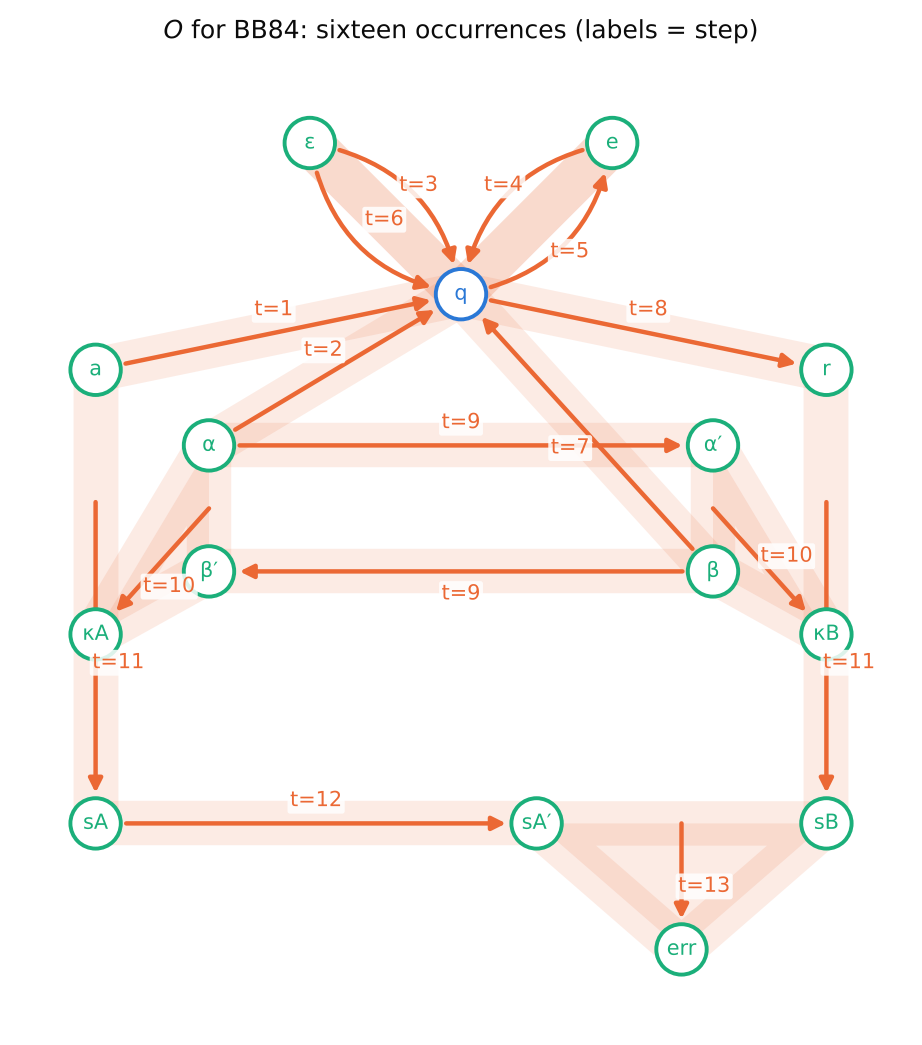
\includegraphics[width=0.7\textwidth]{figs_gluing/g5_bb84_O.png}

\textit{Figure 5. The occurrence hypergraph of BB84 with Eve; labels give the step of each occurrence. The two arcs between $\varepsilon$ and $q$ are Eve's two Hadamards; the two arcs between $q$ and $e$ are her measurement and her resending.}
\end{center}

Under the vertex-set rule, applied to $U(O)$, both pairs are identified: $R$ has fourteen relations, two of multiplicity $2$, and $I_R=0$. Under the directed rule, only Eve's two Hadamards are identified, since the measurement and the resending have opposite directions: $R$ has fifteen relations, one of multiplicity $2$, and $I_R=(t_{qe}-t_{eq})$, with $\beta_{0,0}=1$, $\beta_{1,2}=1$. The term rule gives the same $R$ as the directed rule here, because the two Hadamards carry the same term. In the directed case the remaining generator relates two relations of opposite directions, which the ordinary toric ideal cannot tell apart.

\begin{center}
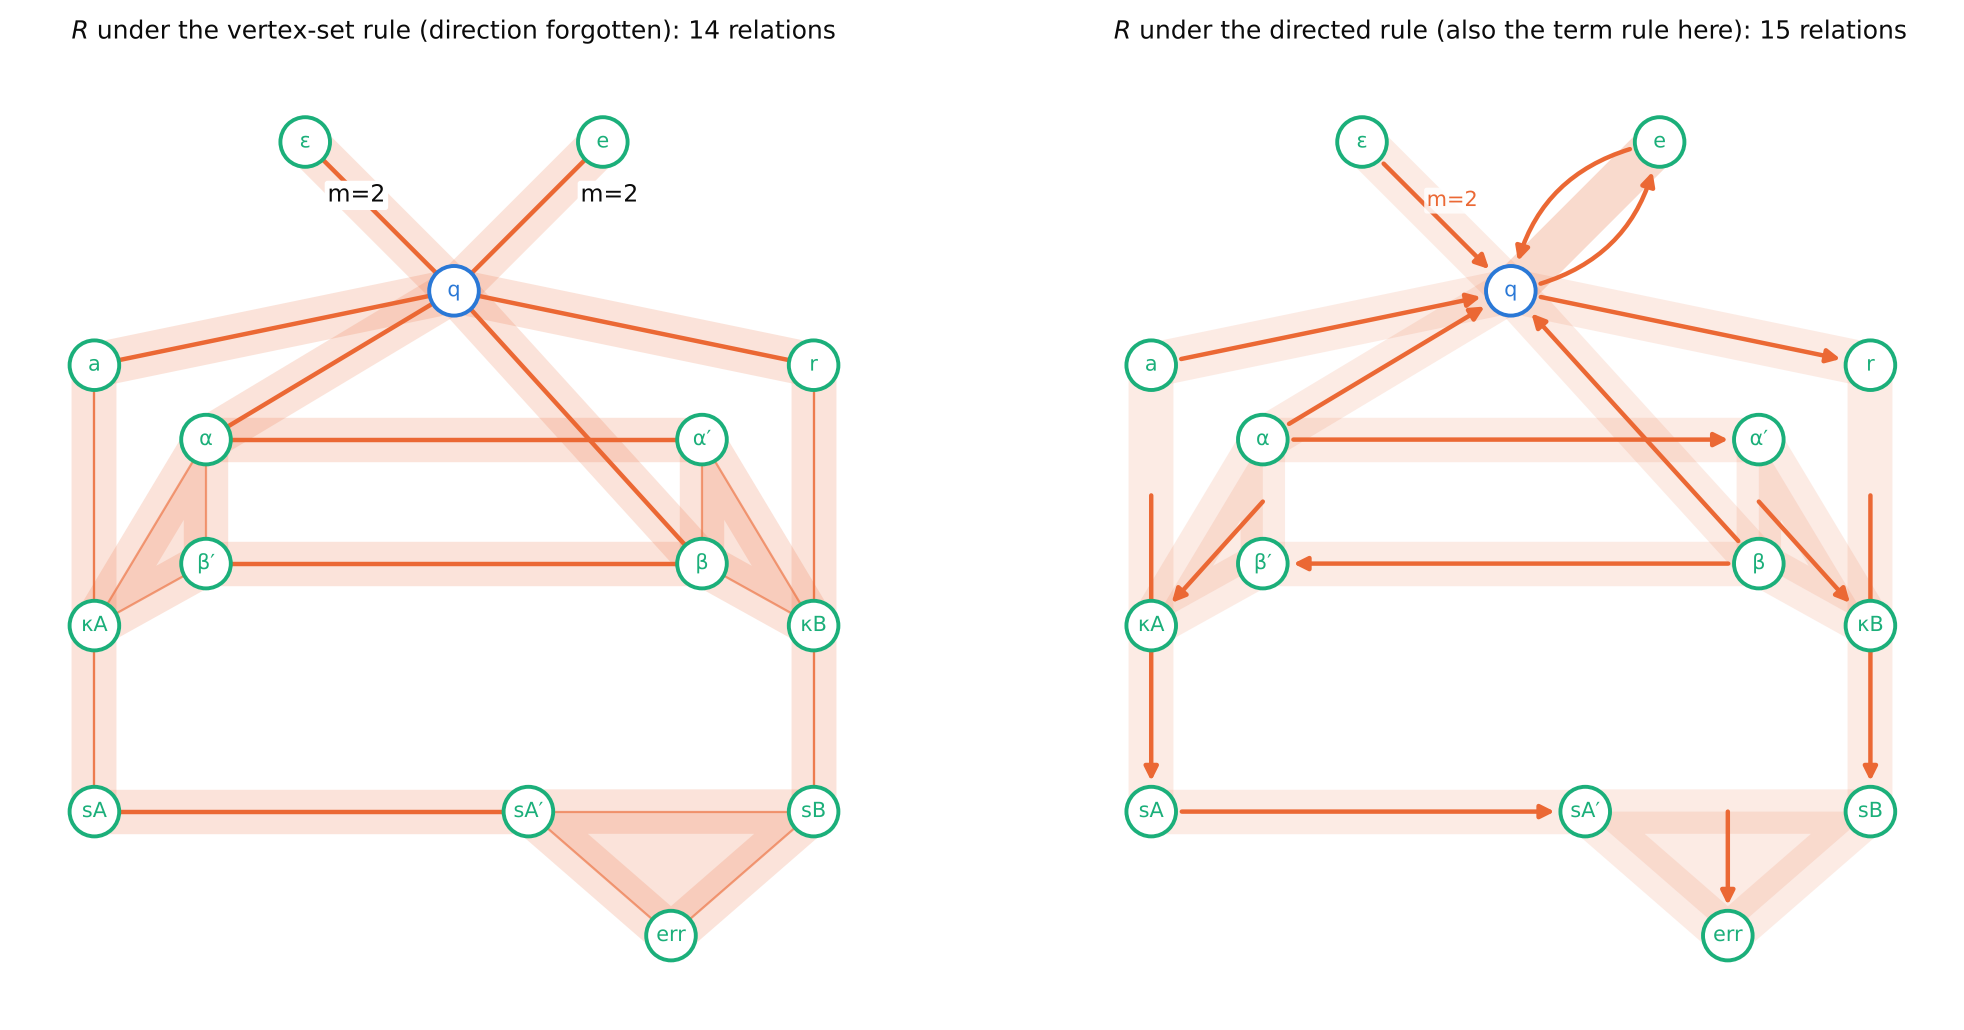
\includegraphics[width=\textwidth]{figs_gluing/g6_bb84_R.png}

\textit{Figure 6. The relation hypergraph of BB84 under the vertex-set rule (left, direction forgotten) and under the directed rule (right); $m$ is the multiplicity of a relation.}
\end{center}

\begin{center}
\begin{tabular}{lllll}
\hline
example & rule & $|E(R)|$ & generators of $I_R$ & nonzero $\beta_{i,j}$\\
\hline
BFS $C_4$ / domino & all & $3$ / $5$ & none & $\beta_{0,0}$\\
teleportation & all & $8$ & one, degree $8$ & $\beta_{0,0},\beta_{1,8}$\\
BB84, $O$ itself & -- & $16$ & two linear binomials & $\beta_{0,0},\beta_{1,2}{=}2,\beta_{2,4}$\\
BB84 & vertex-set & $14$ & none & $\beta_{0,0}$\\
BB84 & directed, term & $15$ & $t_{qe}-t_{eq}$ & $\beta_{0,0},\beta_{1,2}$\\
\hline
\end{tabular}
\end{center}

All ideals and Betti numbers were computed exactly with Macaulay2 over $\mathbb{Q}$.

\subsection{What the construction shows at layer 1}

In the three runs, the relations among relations of layer $1$ over the whole algorithm are few, and they are of two kinds. In BFS there are none: the occurrences form a tree, while the input graph of layer $0$ does carry relations. In teleportation there is exactly one, a balanced collection that involves every kind of operation of the protocol: the gates, both measurements, both sendings and both corrections. In BB84 every relation of $O$ comes from two occurrences on the same vertex set, all of them Eve's, and identifying occurrences by vertex set removes all of them; identifying them by direction leaves only the measurement and resending pair, which differs only in direction. What these facts say about the behaviour of the three algorithms is not addressed here.

\end{document}
